% !TeX spellcheck = en_US
% !TeX root = DynELA.tex
%
% LaTeX source file of DynELA FEM Code
%
% (c) by Olivier Pantalé 2020
%
\chapter{DynELA programming language}

\startcontents[chapters]
\printmyminitoc[2]\LETTRINE{T}his chapter deals about the \DynELA programming language. This language is based on Python 3 and all models must be described using this formalism. Therefore, this chapter will describe step by step how to build a Finite Element Model for the \DynELA, using the Python 3 language. To set-up a model in DynELA, a good knowledge of the Python's 3 language is not mandatory, but it will help to be skillful concerning this language. On the other hand advanced features can be setup with the help of Python 3 language.

\section{Introduction and basic knowledge}
The Python 3 language serves as a support for describing FEM in DynELA. Construction of the Finite Element Model is done by calling some \Cpp methods of the DynELA library through Python language. In fact, the \Cpp methods of the DynELA library are encapsulated by the help of SWIG. Some methods of the DynELA library have therefore been encapsulated using the SWIG utility and are directly accessible from the Python language.

\subsection{Calling the python interpreter}

After the installation and compilation phase of the code\footnote{See the installation instructions in chapter \ref{Chapter!Installation} of the preamble, page \pageref{Chapter!Installation}}, the \DynELA can be used using the following command:

\begin{BashListing}
python model.py
\end{BashListing}

where \textsf{model.py} is the Python 3 source file defining the Finite Element Model. The \textsf{model.py} file contains the definition of the Finite Element Model using a Python 3 language and calls to specific DynELA methods written in \Cpp. The formalism used to set up this Python source file are described is the subsequent chapters.

\subsection{Formalism of a DynELA python file}

To build a Finite Element Model, it is mandatory to import the \textsf{dnlPython} interpreter from the \textsf{.py} script. Conforming to this formalism, we give hereafter the minimal piece of Python code to set up a Finite Element Model in the \DynELA.\index[PL]{dnlPython}

\begin{PythonListing}
#!/usr/bin/env python3
import dnlPython as dnl # Imports the dnlPython library as dnl
model = dnl.DynELA()    # Creates the main Object
...                     # Set of instructions to build the FE model
...                     # conforming to the DynELA language and Python 3
model.solve()           # Runs the solver
...                     # Set of instructions to postprocess the FE model
\end{PythonListing}

In the preceding piece of code, line 2 is used to load into the namespace \textsf{dnl} the \textsf{dnlPython} module containing the interface to all \Cpp methods of the \DynELA, based on the use of the SWIG Python interface. Of course, and conforming to the \textsf{import} command, any name can be used as a namespace to import the DynELA top library. Therefore, all public methods of the \DynELA written in \Cpp can be called from the Python script to build the Finite Element Model, launch the solver, produce output results,\ldots

In the proposed piece of code, line 3 is used to create an object of type \textsf{DynELA} (the higher object type in the \DynELA library) and instantiate it as the \textsf{model} object\footnote{For the rest of this chapter, we assume that the name of the instantiated \textsf{DynELA} object is \textsf{model}.}, while line 6, the solver of the \DynELA library is called to solve the problem and produce the results.

It is also possible, but not recommended, to use the following syntax for lines 2 and 3 of the previous block:
\begin{PythonListing}
#!/usr/bin/env python3
from dnlPython import * # Imports the dnlPython library in current namespace
model = DynELA()        # Creates the main Object
...                     # Rest of the source code defining the FE model
\end{PythonListing}
and then access all top methods and object of the DynELA library directly without referring to the namespace, such as what is proposed in line 3 of the previous block.

As the interpreter of the \DynELA is based on Python 3 language, we can use all instructions valid in Python 3 along with the specific DynELA instructions. In the rest of this documentation, we assume that the notions of programming in Python are mastered, and we will focus only on the functions specific to the \DynELA.


\section{Model, Nodes and Elements}

All Finite Element Models involves nodes and elements. The very first part of the model is therefore to create the nodes and the elements of the structure to set up a Finite Element Model. The \DynELA library doesn't include any meshing procedure yet, therefore, it is mandatory to create all elements and all nodes by hand or using Python loops in case it can be used.

Another way is to use an external meshing program and convert the output of this program to produce the ad hoc lines of Python to describe the elements and the nodes of the model. This has been used many times by the author, and the Abaqus Finite Element code is an efficient way to create the mesh using the \textsf{.inp} text file generated by the CAE Abaqus program and then convert the nodes and elements description parts of the Abaqus inp file into DynELA formalism.

\subsection{Model}

Definition of a model in the \DynELA is done by creating an instance of the \textsf{DynELA} object into memory. This is done by calling the \textsf{dnlPython.DynELA(string)} method that returns an object of type \textsf{DynELA} as presented hereafter.\index[PL]{dnlPython!DynELA(string)}

\begin{PythonListing}
import dnlPython as dnl       # Imports the dnlPython library as dnl
model = dnl.DynELA('Taylor')  # Creates the main Object model named Taylor
\end{PythonListing}

In line 2 of the preceding piece of code, a reference name\footnote{The reference name is a string used to identify the object, this is completely optional but useful for debugging purposes for example as one can know the associated name to an object.} \textsf{Taylor} is associated to the \textsf{model} object during creation. Once the model is created, one can then define all nodes, elements, materials, constitutive laws, boundary conditions,\ldots

\subsection{Nodes}

\subsubsection{Definition of the nodes}

In the \DynELA, creation of nodes is done by calling the \textsf{DynELA::createNode()} method. Therefore, a node is created by calling the \textsf{createNode()} method and giving the new node number and the $x$, $y$ and $z$ coordinates of the new node as presented just below.\index[PL]{DynELA!createNode(int, float, float, float)}

\begin{PythonListing}
model.createNode(1, 0.0, 0.0, 0.0)  # Creates node 1, coordinates [0.0, 0.0, 0.0]
model.createNode(2, 1.0, 2.0, -1.0) # Creates node 2, coordinates [1.0, 2.0, -1.0]
\end{PythonListing}

An alternative method can be used if the coordinates of the node are already stored into a Vec3D object as presented hereafter.\index[PL]{DynELA!createNode(int, Vec3D)}

\begin{PythonListing}
vect = dnl.Vec3D(1.0, 2.0, -1.0) # Creates a Vec3D object [1.0, 2.0, -1.0]
model.createNode(1, vect)        # Creates node 1 with coordinates vect
\end{PythonListing}

A check of the total number of nodes of the structure can be done using the \textsf{DynELA.getNodesNumber()} method that returns the total number of nodes created.

\subsubsection{Definition of the Nodes sets}

Manipulation of nodes, application of boundaries conditions, etc,\ldots is done through the definition of nodes sets. Such nodes sets are used to group nodes under a \textsf{NodeSet} object for further use. A \textsf{NodeSet} object contains a reference name and a list of nodes. Creation of a \textsf{NodeSet} is done using the \textsf{DynELA.NodeSet()} method that returns an new \textsf{NodeSet} instance. The \textsf{NodeSet} can be named during the creation by specifying its name as a string.\index[PL]{NodeSet(string)}

\begin{PythonListing}
nset = dnl.NodeSet('NS_All')
\end{PythonListing}

When the \textsf{NodeSet} has been created, one can now define the list of nodes constituting the \textsf{NodeSet} with the generic \textsf{DynELA.add()} method with the following formalism:

\textsf{DynELA.add(nodeset, start, end, increment)}

Hereafter is some self explaining examples to illustrate this process.

\begin{PythonListing}
nset = dnl.NodeSet('NS_All')
model.add(nset, 2)       # Add node number 2 to node set
model.add(nset, 1, 4)    # Add nodes number 1-4 to node set
model.add(nset, 1, 4, 2) # Add nodes number 1 and 3 to node set
\end{PythonListing}

\subsection{Elements}

\subsubsection{Definition of the elements}

Creation of elements is done by calling the \textsf{DynELA.createElement()} method. An element is created by calling the \textsf{createNode()} method and giving the new element number and the list of nodes defining the element shape separated by comas and ordered thanks to the element definition as presented just hereafter.

\textsf{DynELA.createElement(elementNumber, node1, node2,\ldots)}

Before creating the very first element of the structure, it is necessary to define the element shape using the \textsf{DynELA.setDefaultElement()} method. An example of element creation combining the two preceding methods is presented hereafter.\index[PL]{DynELA!setDefaultElement(Element)}\index[PL]{DynELA!createElement(int, int, int,...)}

\begin{PythonListing}
model.setDefaultElement(dnl.Element.ElQua4N2D) # Defines the default element
model.createElement(1, 1, 2, 3, 4)             # Creates element 1 with nodes 1,2,3,4
\end{PythonListing}

The following elements are available in the \DynELA.
\begin{description}
\item [ElQua4n2D]: 4 nodes bi-linear 2D quadrilateral element.
\item [ElQua4NAx]: 4 nodes bi-linear axisymmetric quadrilateral element.
\item [ElTri3N2D]: 3 nodes 2D triangular element.
\item [ElHex8N3D]: 8 nodes 3D hexahedral element.
\item [ElTet4N3D]: 4 nodes 3D tetrahedral element.
\item [ElTet10N3D]: 10 nodes 3D tetrahedral element.
\end{description}
The total number of elements of the structure can be checked using the \textsf{DynELA.getElementsNumber()} method that returns the total number of elements created.

\subsubsection{Definition of the Element sets}

Declaration of materials, boundaries conditions, etc\ldots is done through the definition of elements sets. Such elements sets are used to group elements under an \textsf{ElementSet} object for further use. An \textsf{ElementSet} object contains a reference to a name and a list of elements. Creation of an \textsf{ElementSet} is done using the \textsf{DynELA.ElementSet()} method that returns a new \textsf{ElementSet} instance. The \textsf{ElementSet} can be named during the creation by specifying its name as a string.

\begin{PythonListing}
eset = dnl.ElementSet('ES_All')
\end{PythonListing}

When the \textsf{ElementSet} has been created, one can now define the list of elements constituting the \textsf{ElementSet} with the generic \textsf{DynELA.add()} method according to the following formalism:

\textsf{DynELA.add(elementset, start, end, increment)}

Hereafter is some self explaining examples to illustrate this process.

\begin{PythonListing}
eset = dnl.ElementSet('ES_All')
model.add(eset, 2)       # Add element number 2 to element set
model.add(eset, 1, 4)    # Add elements number 1-4 to element set
model.add(eset, 1, 4, 2) # Add elements number 1 and 3 to element set
\end{PythonListing}

\subsection{Coordinates transformations}

When the mesh has been created, it is always possible to modify the geometry of the structure by applying some geometrical operations such as translations, rotations and change of scale. Those operations apply on a \textsf{NodeSet}.

\subsubsection{Translations}

One can define a translation of the whole model or a part of the model by defining a translation vector (an instance of the \DynELA \textsf{Vec3D}) and apply this translation to the whole structure (without specifying the \textsf{NodeSet}) or a \textsf{NodeSet} using the \textsf{DynELA.translate()} method with the following syntax.

\begin{PythonListing}
vector = dnl.Vec3D(1, 0, 0)   # Defines the translation vector
model.translate(vector)       # Translates the whole model along [1, 0, 0]
model.translate(vector, nset) # Translates the NodeSet nset along [1, 0, 0]
\end{PythonListing}

\subsubsection{Rotations}

One can define a rotation of the whole model or a part of the model by defining a rotation vector (global axes $\overrightarrow{\ensuremath{x}}$, $\overrightarrow{y}$, $\overrightarrow{\ensuremath{z}}$ or an instance of the \DynELA \textsf{Vec3D}) and an angle $\alpha$ then apply this rotation to the whole structure (without specifying the \textsf{NodeSet}) or a \textsf{NodeSet} using the \textsf{DynELA.rotate()} method with the following syntax.

\begin{PythonListing}
model.rotate('X', angle)        # Rotation of the whole structure around X
model.rotate('X', angle, nset)  # Rotation of NodeSet nset around X
axis = dnl.Vec3D(1.0, 1.0, 1.0) # Defines the axis of rotation
model.rotate(axis, angle)       # Rotation of the whole structure around axis
model.rotate(axis, angle, nset) # Rotation of NodeSet nset around axis
\end{PythonListing}

\subsubsection{Scaling}

One can define a scaling of the whole model or a part of the model by defining a scale factor or a scale vector (an instance of the \DynELA \textsf{Vec3D}) and apply this scaling operation to the whole structure (without specifying the \textsf{NodeSet}) or a \textsf{NodeSet} using the \textsf{DynELA.scale()} method with the following syntax.

\begin{PythonListing}
model.scale(value)             # Scales the whole structure by factor value
model.scale(value, nset        # Scales the NodeSet nset by factor value
vec = dnl.Vec3D(2.0, 1.0, 1.0) # Defines the scale vector
model.scale(vec)               # Scales the whole structure by a factor of 2.0 on x
model.scale(vec, nset)         # Scales the NodeSet nset by a factor of 2.0 on x
\end{PythonListing}

\section{Materials}

\subsection{Declaration of materials}

\subsubsection{Material declaration}

Creation of a Material is done using the \textsf{DynELA.Material()} method. It is possible to give a name to a material during the creation process by specifying it through a string during the declaration. This can be used further.

\begin{PythonListing}
# Creates the material
steel = dnl.Material('Steel')
\end{PythonListing}

\subsubsection{General properties of materials}

General properties of materials in \DynELA concerns the general constants such as Young's modulus, Poisson's ratio, density,\ldots The complete list of parameters is reported in Table \ref{tab:Programming!GeneralProperties}.
\begin{table}[h]
	\begin{center}\begin{tcolorbox}[width=.75\textwidth,myTab,tabularx={l|c|c|R}]
			\multicolumn{1}{c|}{Name} & Symbol & Unit & \multicolumn{1}{c}{Description} \\ \hline\hline
			youngModulus & $E$ & $MPa$ & Young modulus\\
			poissonRatio & $\nu$ &  & Poisson ratio\\
			density & $\rho$ & $kg/m^3$ & Density\\
			heatCapacity & $C_{p}$ & $J/^{\circ}C$ & Heat capacity\\
			taylorQuinney& $\eta$ & & Taylor-Quinney coefficient\\
			initialTemperature & $T_{0}$ & $^{\circ}C$ & Initial temperature
	\end{tcolorbox}\end{center}\caption{General properties of materials\label{tab:Programming!GeneralProperties}}
\end{table}
After creating an instance of the object \textsf{dnl.Material}, on can apply the prescribed values to all those parameters using the following syntax.

\begin{PythonListing}
# Creates the material
steel = dnl.Material('Steel')
# Apply all parameters
steel.youngModulus = 206e9
steel.poissonRatio = 0.3
steel.density = 7830
steel.heatCapacity = 46
steel.taylorQuinney = 0.9
steel.initialTemperature = 25
\end{PythonListing}

\subsubsection{Material affectation to a set of elements}

And, the material can be affected to the elements of the model by the \textsf{DynELA.add()} method as proposed hereafter.

\begin{PythonListing}
# Creates the material
steel = dnl.Material('Steel')
# Apply all parameters
...
# Affect the material to the element set eset
model.add(steel, eset)
\end{PythonListing}

\subsection{Johnson-Cook constitutive law}

The Johnson-Cook constitutive law is an hardening law defining the yield stress $\sigma^{y}(\overline{\varepsilon}^{p},\stackrel{\bullet}{\overline{\varepsilon}^{p}},T)$ by the following equation:

\begin{equation}
\sigma^{y}=\left(A+B\overline{\varepsilon}^{p^{n}}\right)\left[1+C\ln\left(\frac{\stackrel{\bullet}{\overline{\varepsilon}^{p}}}{\stackrel{\bullet}{\overline{\varepsilon}_{0}}}\right)\right]\left[1-\left(\frac{T-T_{0}}{T_{m}-T_{0}}\right)^{m}\right]
\end{equation}
where $\stackrel{\bullet}{\overline{\varepsilon}_{0}}$ is the reference strain rate, $T_{0}$ and $T_{m}$ are the reference temperature and the melting temperature of the material respectively and $A$, $B$, $C$, $n$ and $m$ are the five constitutive flow law parameters. Therefore, this kind of hardening law can be defined by using the following piece of code:

\begin{PythonListing}
hardLaw = dnl.JohnsonCookLaw()                       # Hardening law
hardLaw.setParameters(A, B, C, n, m, depsp0, Tm, T0) # Parameters of the law
\end{PythonListing}

Once the hardening law has been created, one have to link this hardening law to a material already defined using the following piece of code:

\begin{PythonListing}
# Creates the material
steel = dnl.Material('Steel')
# Creates the hardening law
hardLaw = dnl.JohnsonCookLaw()
# Attach hardening law to material
steel.setHardeningLaw(hardLaw)
\end{PythonListing}

\section{Boundaries conditions}

\subsection{Restrain boundary condition}

\begin{PythonListing}
# Declaration of a boundary condition for top part
topBC = dnl.BoundaryRestrain('BC_top')
topBC.setValue(0, 1, 1)
model.attachConstantBC(topBC, topNS)
\end{PythonListing}

\subsection{Amplitude}

\begin{PythonListing}
# Declaration of a ramp function to apply the load
ramp = dnl.RampFunction('constantFunction')
ramp.set(dnl.RampFunction.Constant, 0, stopTime)
\end{PythonListing}

\subsection{Constant speed}

\begin{PythonListing}
# Declaration of a boundary condition for top part
topSpeed = dnl.BoundarySpeed()
topSpeed.setValue(displacement, 0, 0)
topSpeed.setFunction(ramp)
model.attachConstantBC(topSpeed, topNS)
\end{PythonListing}

\subsection{Initial speed}

\begin{PythonListing}
# Declaration of a ramp function to apply the load
ramp = dnl.RampFunction('constantFunction')
ramp.set(dnl.RampFunction.Constant, 0, stopTime)
\end{PythonListing}

\section{Fields}\label{ProgrammingLanguage:Section:Fields}

\subsection{Nodal fields}

Nodal fields are defined at nodes and cover types defined in table \ref{tab:Programming!NodalFields}. Concerning those fields, some of them are directely defined at nodes, some other are extrapolated from integration points and transfered to nodes as reported in column \textsf{loc} of table \ref{tab:Programming!NodalFields}. Concerning types, \textsf{scalars}, \textsf{vec3D} and \textsf{tensors} are available. Depending in the type of data, different methods can be used to acces those data:
\begin{description}
	\item [{scalar}] : Direct access to the value as it is unique.
	\item [{vec3D}] : Access to all $3$ components of a vec3D using \textsf{nameX}, \textsf{nameY}, \textsf{nameZ} or the norm of the vec3D using \textsf{name}.
	\item [{tensor}] : Access to all $9$ components of a tensor using \textsf{nameXX}, \textsf{nameXY},\ldots, \textsf{nameZZ} or the norm of the tensor using \textsf{name}.
\end{description}
\begin{table}[h]
	\begin{center}\begin{tcolorbox}[width=.85\textwidth,myTab,tabularx={l|c|c|c|c|R}]
			\multicolumn{1}{c|}{Name} & & Type & nb & Loc & \multicolumn{1}{c}{Description} \\ \hline\hline
			density & $\rho$ & scalar & $1$ & IntPt &\\ \hline
			displacementIncrement & $\Delta\overrightarrow{u}$ & vec3D & $3+1$ & node & \\ \hline
			displacement & $\overrightarrow{u}$ & vec3D & $3+1$ & node & \\ \hline
			energyIncrement && scalar & $1$ & IntPt & \\ \hline
			energy && scalar & $1$ & IntPt & \\ \hline
			gammaCumulate && scalar & $1$ & IntPt & \\ \hline
			gamma & $\Gamma$ & scalar & $1$ & IntPt & \\ \hline
			internalEnergy && scalar & $1$ & IntPt & \\ \hline
			mass & $m$ & scalar & $1$ & node & \\ \hline
			nodeCoordinate & $\overrightarrow{x}$ & vec3D & $3+1$ & node & \\ \hline
			normal & $\overrightarrow{n}$ & vec3D & $3+1$ & node & \\ \hline
			PlasticStrainInc && tensor & $9+1$ & IntPt & \\ \hline
			plasticStrainRate && scalar & $1$ & IntPt & \\ \hline
			plasticStrain && scalar & $1$ & IntPt & \\ \hline
			PlasticStrain && tensor & $9+1$ & IntPt & \\ \hline
			pressure & $p$ & scalar & $1$ & IntPt & \\ \hline
			speedIncrement & $\Delta\overrightarrow{v}$ & vec3D & $3+1$ & node & \\ \hline
			speed & $\overrightarrow{v}$ & vec3D & & node & \\ \hline
			StrainInc && tensor & $9+1$ & IntPt & \\ \hline
			Strain && tensor & $9+1$ & IntPt & \\ \hline
			Stress & $\Sig$ & tensor & $9+1$ & IntPt & \\ \hline
			temperature & $T$ & scalar & $1$ & IntPt & \\ \hline
			vonMises & $\overline{\sigma}$ & scalar & $1$ & IntPt & \\ \hline
			yieldStress & $\sigma^y$ & scalar & $1$ & IntPt &
	\end{tcolorbox}\end{center}\caption{Nodal fields\label{tab:Programming!NodalFields}}
\end{table}

\subsection{Element fields}

Element fields are defined at integration points and cover types defined in table \ref{tab:Programming!ElementlFields}. Concerning types, \textsf{scalars}, \textsf{vec3D} and \textsf{tensors} are available. Depending in the type of data, different methods can be used to acces those data:
\begin{description}
	\item [{scalar}] : Direct access to the value as it is unique.
	\item [{vec3D}] : Access to all $3$ components of a vec3D using \textsf{nameX}, \textsf{nameY}, \textsf{nameZ} or the norm of the vec3D using \textsf{name}.
	\item [{tensor}] : Access to all $9$ components of a tensor using \textsf{nameXX}, \textsf{nameXY},\ldots, \textsf{nameZZ} or the norm of the tensor using \textsf{name}.
\end{description}
\begin{table}[h]
	\begin{center}\begin{tcolorbox}[width=.85\textwidth,myTab,tabularx={l|c|c|c|R}]
			\multicolumn{1}{c|}{Name} && Type & nb & \multicolumn{1}{c}{Description} \\ \hline\hline
			density & $\rho$ & scalar & $1$ & \\ \hline
			gammaCumulate && scalar & $1$ & \\ \hline
			gamma & $\Gamma$ & scalar & $1$ & \\ \hline
			internalEnergy && scalar & $1$ & \\ \hline
			plasticStrainRate && scalar & $1$ & \\ \hline
			plasticStrain && scalar & $1$ & \\ \hline
			PlasticStrain && tensor & $9+1$ & \\ \hline
			PlaticStrainInc && tensor & $9+1$ & \\ \hline
			pressure & $p$ & scalar & $1$ & \\ \hline
			StrainInc && tensor & $9+1$ & \\ \hline
			Strain && tensor & $9+1$ & \\ \hline
			Stress & $\Sig$ & tensor & $9+1$ & \\ \hline
			temperature & $T$ & scalar & $1$ & \\ \hline
			vonMises & $\overline{\sigma}$ & scalar & $1$ & \\ \hline
			yieldStress & $\sigma^y$ & scalar & $1$ &
	\end{tcolorbox}\end{center}\caption{Element fields\label{tab:Programming!ElementlFields}}
\end{table}

\subsection{Global fields}

\begin{table}[h]
	\begin{center}\begin{tcolorbox}[width=.85\textwidth,myTab,tabularx={l|c|c|c|R}]
			\multicolumn{1}{c|}{Name} && Type & nb & \multicolumn{1}{c}{Description} \\ \hline\hline
			kineticEnergy & $E_c$ & scalar & $1$ & \\ \hline
			realTimeStep & $\Delta t_r$ & scalar & $1$ & \\ \hline
			timeStep &$\Delta t$& scalar & $1$ &
	\end{tcolorbox}\end{center}\caption{Global fields\label{tab:Programming!GlobalFields}}
\end{table}

\section{Data Output during computation}

\subsection{VTK Data files}
The \DynELA is able to export results in VTK (The Visualization Toolkit\footnote{See : https://vtk.org}) ASCII files. Those files can be used to visualize the results of computations using the Paraview post-processing software\footnote{See : https://www.paraview.org}.

Those VTK files are automatically created during the solving phase. Controlling the instant of file save is done using the following syntax:\index[PL]{DynELA!setSaveTimes(float, float, float)}
\begin{PythonListing}
model.setSaveTimes(startTime, stopTime, incrementTime)
\end{PythonListing}
where \textsf{startTime}, \textsf{stopTime}, \textsf{incrementTime} are $3$ times defining respectively the times of the first file, the last one and the period of time between subsequent frames.

At any time, it is possible to export a VTK file using the method \textsf{writeVTKFile( )}\index[PL]{DynELA!writeVTKFile( )} of the \textsf{DynELA} class.

\subsection{History files}

During the solving procedure, one can export time history datafiles that can be used to produce time-history plots. This kind of files are text files in CSV format directly exported from the DynELA solver. In order to control the production of those files, one have to create an instance of the \textsf{HistoryFile} class and add this instance to the current model. Those history-files can then be used to produce high-quality plots through the associated \textsf{Curves Utility} of the \DynELA presented in chapter \ref{chap:CU!CU}, or use the produced data-file in any external plotting application.

As an illustration, the following commented piece of code has been used to produce the CSV history file reported in Figure \ref{fig:PL!HF!Export}.
\begin{PythonListing}
hist = dnl.HistoryFile()              # Constructor of the hist object
hist.setFileName('HistoryPlot.plot')  # Sets the filename of the history file
hist.add(dnl.Field.timeStep)                 # First column will be timeStep value
hist.add(histES, 0, dnl.Field.vonMises)      # Second one will be von Mises stress
hist.add(histRad, dnl.Field.nodeCoordinateX) # Third one will be X node coordinate
hist.setSaveTime(1e-6)                       # One data every 1E-6 s
model.add(hist)                              # Add the time history to the solver
\end{PythonListing}

\begin{figure}[h]
\begin{centering}
\begin{BashListing}
#DynELA FEM Code v. 4.0 history file
#plotted :timeStep vonMises nodeCoordinateX
0.0000000E+00 6.2463483E-08 0.0000000E+00 3.2000000E+00
1.0623148E-06 6.2462797E-08 1.3439840E+03 3.5412151E+00
2.0617159E-06 6.2462515E-08 1.3643205E+03 3.7516529E+00
3.0611173E-06 6.2462676E-08 1.3748692E+03 3.9635932E+00
4.0605220E-06 6.2462901E-08 1.3662499E+03 4.1161636E+00
5.0599347E-06 6.2465035E-08 1.3539346E+03 4.2812566E+00
.....
\end{BashListing}
\par\end{centering}
\caption{Export of a CSV history file\label{fig:PL!HF!Export}}
\end{figure}

In file reported in Figure \ref{fig:PL!HF!Export}, the first two lines are comments. Line $1$ shows the name and version of the \DynELA while line $2$ shows the name of the fields from columns 2 to the end of the table (in this example, current time is in column 1, time-step $\Delta t$ is in column 2, von Mises stress $\overline{\sigma}$ at the center of the element referred by element-set \emph{histES} is in column 3 and nodal coordinate $x$ of the node defined in \emph{histRad} node-set is in the last column of the table). One data is more or less produced at each requested time ($t_i=10^{-6}s$), but this depends on the time-step increment $\Delta t$ of the Explicit solver.

\subsubsection{Definition of data to save}

\begin{description}
\item [{add (\emph{ElementSet}, \emph{int}, \emph{field})}] : Add the output data \emph{field} defined at integration point \emph{int} for all elements defined in the element-set \emph{ElemenSet} to the current time-history plot.\index[PL]{HistoryFile!add(ElementSet)}
\item [{add (\emph{NodeSet}, \emph{Field})}] : Add the output data \emph{Field} for all nodes defined in the node-set \emph{NodeSet} to the current time-history plot.\index[PL]{HistoryFile!add(NodeSet)}
\item [{add (\emph{Field})}] : Add the global \emph{Field} value to the current time-history plot.\index[PL]{HistoryFile!add(Field)}
\item [{setFileName (\emph{string})}] : Defines the name of the output CSV filename.\index[PL]{HistoryFile!setFileName(string)}
\item [{setSaveTime (\emph{float})}] : Defines the frequency of data store during the computation.\index[PL]{HistoryFile!setSaveTime(float)}
\item [{setSaveTime (\emph{float}[start], \emph{float}[stop], \emph{float}[freq])}] : Defines the start, stop and frequency of data store during the computation starting at \emph{start}, ending at \emph{stop} and with the frequency defined by \emph{freq}.\index[PL]{HistoryFile!setSaveTime(float, float, float)}
\end{description}

When data storage has been defined, it is mandatory to add the \textsf{HistoryFile} object created to the \textsf{model} to produce the output files during computation. this is done using the following syntax:\index[PL]{DynELA!add(HistoryFile)}
\begin{PythonListing}
model.add(hist)
\end{PythonListing}
where \emph{model} is the \textsf{model} to solve and \emph{hist} is the requested history-file object.

\subsubsection{Check of data information}
Data information defined in the previous subsection can be checked using one of the following commands:
\begin{description}
\item [{getSaveTime ( )}] : Returns the frequency of data store.\index[PL]{HistoryFile!getSaveTime( )}
\item [{getStartTime ( )}] : Returns the start-time of data store. \index[PL]{HistoryFile!getStartTime( )}
\item [{getStopTime ( )}] : Returns the end-time of data store.\index[PL]{HistoryFile!getStopTime( )}
\item [{getFileName ( )}] : Returns the file name for data store.\index[PL]{HistoryFile!getFileName( )}
\end{description}

\section{Solvers}
The \DynELA currently have only one FEM solver: an Explicit solver based on a Chung-Hulbert algorithm. Declaration of such a solver is done by creating an instance of the \textsf{Explicit} solver class, using the following syntax:
\begin{PythonListing}
solver = dnl.Explicit('Solver') # Declaration of the explicit solver
solver.setTimes(0, stopTime)    # Definition of start and end time
model.add(solver)               # Link solver to the current model
\end{PythonListing}
In this example, we create an explicit solver named solver at line $1$, defines the starting and ending times of the computation at line $2$ and attach the created solver to the current FEM model at line $3$.

The Explicit class contains some useful methods as reported here after:
\begin{description}
\item [{setComputeTimeStepFrequency(\emph{int})}] : Defines the frequency (\ie every how many increments) of re-computing the critical time step of the model.\index[PL]{Solver!setComputeTimeStepFrequency(int)}
\item [{setIncrements(\emph{int}, \emph{int})}] : Defines the start and stop increments for the solver.\index[PL]{Solver!setIncrements(int, int)}
\item [{setTimes(\emph{float}, \emph{float})}] : Defines start and stop time of the current job.\index[PL]{Solver!setTimes(float, float)}
\item [{setTimeStepMethod(\emph{method} )}] : Defines the method used to compute the time-step which can be one of the three following methods: \textsf{Courant}, \textsf{PowerIteration} or \textsf{PowerIterationUnder}.\index[PL]{Solver!setTimeStepMethod(method)}
\item [{setTimeStepSafetyFactor(\emph{float} safetyfactor )}] : Defines the time-step safety factor (normally within the range  $[0:1]$).\index[PL]{Solver!setTimeStepSafetyFactor(float)}
\end{description}

\subsection{Parallel solver}
In \DynELA it is possible to control the number of cores to use for the solver through the \textsf{Parallel} class. If no options are given to the parallel solver, it assumes that only $1$ core will be used for the computation. There are currently few options in the parallel class and the following ones can be used to control the parallelization of the Explicit solver:
\begin{description}
\item [{setCores (\emph{int})}] : Set the number of cores to use for the solver.\index[PL]{parallel!setCores(int)}
\item [{getCores ( )}] : Get the number of cores used by the solver.\index[PL]{parallel!getCores( )}
\end{description}
The control of the number of cores to use in an explicit solve is done using the following syntax, where \textsf{model} refers to the DynELA Finite Element Model.
\begin{PythonListing}
# Parallel solver with two cores
model.parallel.setCores(2)
\end{PythonListing}

\subsection{Solving procedure}
Running solver is done through the \textsf{solve} method of the \textsf{DynELA} class using the following syntax:
\begin{PythonListing}
# Run the main solver
model.solve()
\end{PythonListing}
At the beginning of the solving procedure, a call to the \textsf{initSolve} method of the same \textsf{DynELA} class is performed. It is also possible make a explicit call to the \textsf{initSolve} method (\ie separated from the one hidden in the solve method). This is useful if someone wants to modify values of different fields before running the solver for example\footnote{With such an approach, it is possible for example to modify all the fields of all points of the structure and to input the ones coming from another FEM code for example. It is also possible to modify for example only the temperature of all nodes of the structure thanks to an analytical model and run the solver on the basis of those new temperatures, \ie to make an hybrid FEM/analytical simulation.}.

Commands available for running the solver are the following ones:
\begin{description}
\item [{initSolve ( )}] : Runs the init solve of the \DynELA.\index[PL]{DynELA!initSolve( )}
\item [{solve ( )}] : Runs the solver of the \DynELA.\index[PL]{DynELA!solve( )}
\end{description}


\section{Vectorial SVG meshes and contourplots}
Since \DynELA version 3.0, it is possible to export SVG files (Scalable Vector Graphics) from the Python command language to produce high quality figures (and of course reproducible results, as everything is generated from script). This can be done before running the Solver to export the initial mesh of the structure for example, or after the solver phase to produce contourplot results. One can then produce some mesh exports as presented in Figure \ref{fig:PL!SVG!Mesh} or contourplots exports for a given data (here we used the von Mises field) as presented in Figure \ref{fig:PL!SVG!Contourplot}.
\begin{figure}[h]
\begin{centering}
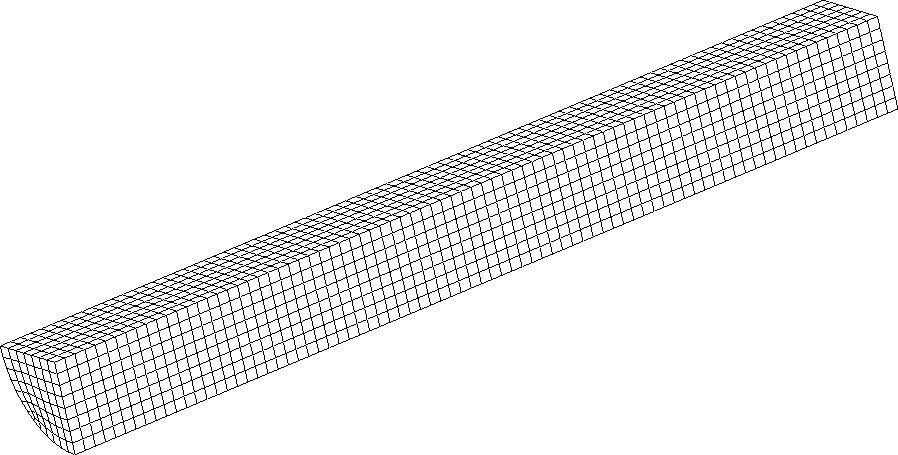
\includegraphics[width=0.5\columnwidth]{Figures/ProgrammingLanguage/mesh}
\par\end{centering}
\caption{Export of a mesh in SVG format\label{fig:PL!SVG!Mesh}}
\end{figure}

\begin{figure}[h]
\begin{centering}
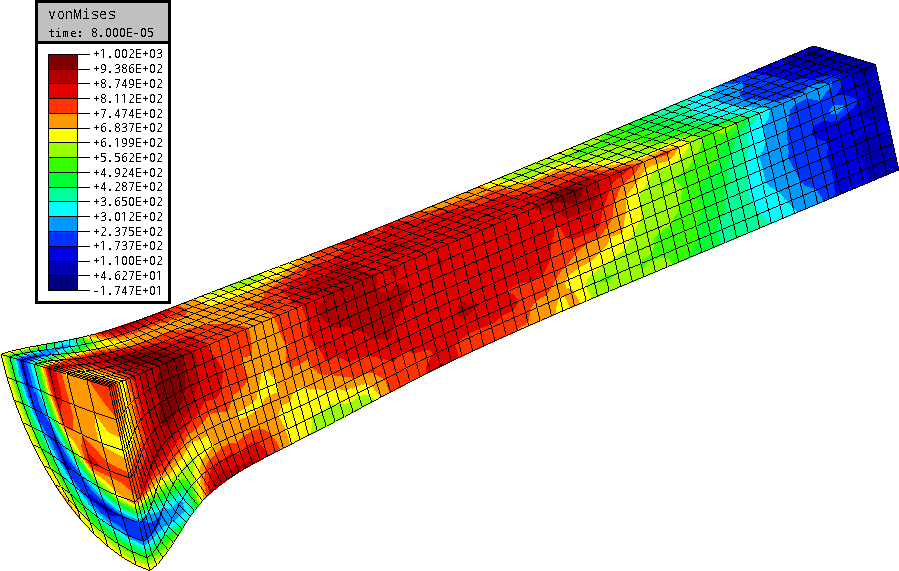
\includegraphics[width=0.5\columnwidth]{Figures/ProgrammingLanguage/vonMisesCP}
\par\end{centering}
\caption{Export of a von Mises contourplot in SVG format\label{fig:PL!SVG!Contourplot}}
\end{figure}

As an illustration, the following commented piece of code has been used to produce both plots presented in Figures \ref{fig:PL!SVG!Mesh} and \ref{fig:PL!SVG!Contourplot}.
\begin{PythonListing}
svg = dnl.SvgInterface('SVG')       # Creates an instance of SvgInterface object
svg.setLegendPosition(100, 280)     # Position the legend
svg.rotate(dnl.Vec3D(0, 1, 0), 190) # Rotation 190 degree around Y axis
svg.rotate(dnl.Vec3D(1, 0, 0), -70) # Rotation -70 degree around X axis
svg.rotate('Y', -60)                # Rotation -60 degree around Y axis
svg.write('mesh.svg')               # Exports the mesh
svg.write('vonMises.svg', dnl.Field.vonMises) # Exports the contourplot
\end{PythonListing}

More details concerning the syntax of the SvgInterface class are presented in the following subsections.

\subsection{Initialization of an SVG object}
Creation of a SVG file under \DynELA is done using through the instantiation of an object \textsf{SvgInterface} object using the following syntax:
\begin{PythonListing}
svg = dnl.SvgInterface('SVG object')
\end{PythonListing}
In this piece of code, \textsf{svg} is an instance of the object \textsf{SvgInterface} and '\emph{SVG object}' is the associated name of the object created by the constructor of the \textsf{SvgInterface} class.

Concerning \textsf{SvgInterface}, \DynELA creates a window with the prescribed size $1600\times1600$, where the coordinates of the top-left corner are $(0, 0)$ and the coordinates of the bottom-right corner are $(1600, 1600)$. All drawing options where some coordinates are requested must conform to this definition.

\subsection{Drawing options}

\subsubsection{View orientation and rotations}
\begin{description}
\item [{resetView ( )}] : This resets the current view to the original one where $O,\overrightarrow{x},\overrightarrow{y}$ is the drawing plane and $\overrightarrow{z}$ is pointing forward.\index[PL]{SvgInterface!resetView( )}
\item [{rotate (\emph{string}, \emph{float})}] : Defines the rotation of the global structure around one of the $3$ base axis referred by the \emph{string} value 'X', 'Y' or 'Z' with an angle $\alpha$ defined by a \emph{float} value.\index[PL]{SvgInterface!rotate(string, float)}
\item [{rotate (\emph{Vec3D}, \emph{float})}] : Defines the rotation of the global structure around the axis $\overrightarrow{v}$ defined by a \emph{Vec3D} with an angle $\alpha$ defined by a \emph{float} value.\index[PL]{SvgInterface!rotate(Vec3D, float)}
\end{description}

\subsubsection{Mesh and data output}
\begin{description}
\item [{setMeshDisplay (\emph{bool} = [true])}] : Set or unset the drawing of the mesh.\index[PL]{SvgInterface!setMeshDisplay(bool)}
\item [{setMeshThickness (\emph{float} = [1.0])}] : Defines the line thickness for drawing the mesh.\index[PL]{SvgInterface!setMeshThickness(float)}
\item [{setPatchLevel (\emph{int} = [1])}] : Defines the level of decomposition of the elements for drawing, \ie the number of recursive decomposition of the polygons [1 to 4]. The default value is usually sufficient for all plots, increasing it enhances the precision of the plot, but drastically increases also the size of the produced file.\index[PL]{SvgInterface!setPatchLevel(int)}
\item [{setAutoRangeValues (\emph{bool} = [true])}] : Set or unset the automatic computation of minimum and maximum values for fields range. This function must be switched to \emph{false} in addition to the function \textsf{setBounds} of the \textsf{colorMap} class (see \ref{sec:PL!SVG!ColorMap}).\index[PL]{SvgInterface!setAutoRangeValues(bool)}
\end{description}

\subsubsection{Legends and notations}
\begin{description}
\item [{setInfoDisplay (\emph{bool} = [false])}] : Set or unset the drawing of the bloc of informations.\index[PL]{SvgInterface!setInfoDisplay(bool)}
\item [{setInfoPosition (\emph{int}, \emph{int})}] : Defines the position of the bloc of informations on the current drawing (default position is $(50, 1200)$).\index[PL]{SvgInterface!setInfoPosition(int, int)}
\item [{setLegendDisplay (\emph{bool} = [true])}] :  Set or unset the drawing of the legend.\index[PL]{SvgInterface!setLegendDisplay(bool)}
\item [{setLegendPosition (\emph{int}, \emph{int})}] : Defines the position of the legend on the current drawing (default position is $(30, 30)$).\index[PL]{SvgInterface!setLegendPosition(int, int)}
\item [{setTitleDisplay (\emph{bool} = [true])}] :  Set or unset the drawing of the title.\index[PL]{SvgInterface!setTitleDisplay(bool)}
\item [{setTitlePosition (\emph{int}, \emph{int})}] : Defines the position of the title on the current drawing (default position is $(50, 1550)$).\index[PL]{SvgInterface!setTitlePosition(int, int)}
\end{description}

\subsubsection{Color Map Options}\label{sec:PL!SVG!ColorMap}
Color Map used for SVG plots can be changed to one of the predefined color-maps using the following syntax (ex: changing for a gray map):
\begin{PythonListing}
svg.colorMap.setGrayMap() # set the color map to Gay
\end{PythonListing}
The following 6 maps are available in \DynELA.
\begin{description}
\item [{setColorMap ( )}] : defines a classic color map.\\
 \hspace*{0.2\columnwidth}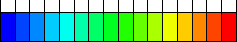
\includegraphics{Figures/ProgrammingLanguage/ColorMap}
\item [{setDeepColorMap ( )}] : defines a deep-color map (this is the \textsf{default} map).\\
 \hspace*{0.2\columnwidth}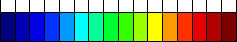
\includegraphics{Figures/ProgrammingLanguage/DeepColorMap}
\item [{setGrayMap ( )}] : defines a gray map.\\
 \hspace*{0.2\columnwidth}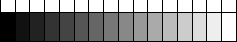
\includegraphics{Figures/ProgrammingLanguage/GrayMap}
\item [{setReverseColorMap ( )}] : defines a reversed classic color map (from red to blue).\\
 \hspace*{0.2\columnwidth}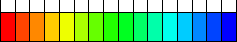
\includegraphics{Figures/ProgrammingLanguage/ReverseColorMap}
\item [{setReverseDeepColorMap ( )}] : defines a reversed deep-color map (from red to blue).\\
 \hspace*{0.2\columnwidth}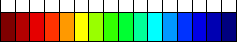
\includegraphics{Figures/ProgrammingLanguage/ReverseDeepColorMap}
\item [{setReverseGrayMap ( )}] : defines a reversed gray map (from white to black).\\
 \hspace*{0.2\columnwidth}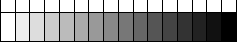
\includegraphics{Figures/ProgrammingLanguage/ReverseGrayMap}
\end{description}

In \DynELA, maps are defined by a given range and number of isovalues. Those parameters can be defined using the following methods:
\begin{description}
\item [{setLevels (\emph{int} = [16]})] : maps are decomposed into the given number of colors, \ie isovalues levels.
\item [{setBounds (\emph{float}, \emph{float})}] : maps are automatically ranged to fit the current field range. But this method allows to fix this range\footnote{In order to use this method it is mandatory to use the method \textsf{setAutoRangeValues} of the \textsf{SvgInterface} class and set it to \emph{false}.}. Out of bounds zones will be drawn in black for low values and white for high values.
\end{description}

On the other hand, the following methods returns some informations on the current map:
\begin{description}
\item [{getMax ( )}] : get the maximum value of the range.
\item [{getMin ( )}] : get the minimum value of the range.
\item [{getLevels ( )}] : get the current number of levels.
\end{description}

\subsection{Creation of the SVG file}
Effective creation of the SVG file is done by calling the \textsf{write} method of the \textsf{SvgInterface} class with the following syntax:\index[PL]{SvgInterface!write(string)}\index[PL]{SvgInterface!write(string, Field)}
\begin{PythonListing}
svg.write('mesh.svg') # Without field, this draws only the mesh
svg.write('temp.svg', dnl.Field.temperature)
\end{PythonListing}
Here, on line number 1, '\emph{temp.svg}' is the name of the SVG file to create for exporting the mesh. On line number 2, '\emph{temp.svg}' is the name of the SVG file to create and \textsf{dnl.Field.temperature} is the name of the associated field to output (see \ref{ProgrammingLanguage:Section:Fields} for definitions).
